\documentclass{article}

\usepackage[T1]{fontenc}
\usepackage[utf8]{inputenc}
\usepackage{microtype}
\usepackage{graphicx}
\usepackage{subcaption}
\usepackage{booktabs}
\usepackage{multirow}
\usepackage{hyperref}

\newcommand{\theHalgorithm}{\arabic{algorithm}}

% Adversarial-selection numbers — multi-seed validation of iter_014
% (the best of four tied in-loop top candidates by both-feasibility
% rate). See results/adversarial_validation.json.
\newcommand{\AdvValSeeds}{5}
\newcommand{\AdvValTrainGapMean}{$-$6.16}
\newcommand{\AdvValTrainGapStd}{8.01}
\newcommand{\AdvValStressGapMean}{$-$1.14}
\newcommand{\AdvValStressGapStd}{2.07}
\newcommand{\AdvValMinGapMean}{$-$5.42}
\newcommand{\AdvValMinGapStd}{6.03}
\newcommand{\AdvValBothFeasPct}{80\%}

\usepackage{icml2026}

\usepackage{amsmath}
\usepackage{amssymb}
\usepackage{mathtools}
\usepackage{amsthm}

\usepackage[capitalize,noabbrev]{cleveref}

\icmltitlerunning{FunWake: A Benchmark for LLM-Discovered Optimization Algorithms}

\begin{document}

\twocolumn[
\icmltitle{FunWake: A Low-Cost Benchmark for\\
LLM-Discovered Optimization Algorithms}

\icmlsetsymbol{equal}{*}

\begin{icmlauthorlist}
\icmlauthor{Anonymous Authors}{anon}
\end{icmlauthorlist}

\icmlaffiliation{anon}{Anonymous Institution}

\icmlcorrespondingauthor{Anonymous Authors}{anon@example.com}

\icmlkeywords{LLM agents, algorithm discovery, wind farm optimization, benchmark}

\vskip 0.3in
]

\printAffiliationsAndNotice{}

\begin{abstract}
Can LLM agents discover novel optimization algorithms, or do they
default to reimplementing known methods? We introduce FunWake, a
benchmark that tests this by exposing two tool interfaces to the same
LLM agent on the same physics problem (wind farm layout optimization).
A \emph{narrow} interface restricts the agent to writing a 4-output
schedule function controlling the learning rate, penalty weight, and
Adam momentum of a fixed gradient optimizer; a \emph{broad} interface
lets the agent write an arbitrary optimization routine from scratch.
Given the narrow interface, agents propose novel schedule
\emph{parameterizations} (dual Gaussian LR bumps, cyclic Adam betas
synchronized with cosine restarts) that generalize across turbine
counts ($N{=}30$ to $300$) and to a physics-distinct held-out farm;
ablations show non-LLM search inside the proposed parameter family
matches the LLM's scores, isolating the LLM's contribution to
parameterization design rather than numerical tuning. Given the broad
interface, agents converge on reimplementing community-standard
solvers (SLSQP) with better initialization, valid engineering but not
new algorithmic knowledge. FunWake evaluates on CPU in
30--45\,s per candidate at training scale ($N{=}50$) and scales
predictably (340\,s at $N{=}200$; SLSQP exceeds 1600\,s at the same
size), making iterative search practical at workshop budgets.
\end{abstract}

\section{Benchmark Design}

\paragraph{Problem.}
Place $N$ wind turbines inside a polygon to maximize annual energy
production (AEP) subject to boundary and minimum-spacing constraints,
using a differentiable Gaussian wake
model~\cite{bastankhah2014new} implemented in JAX.

\paragraph{Two interfaces.}
In \emph{schedule-only} mode, the LLM writes
\texttt{schedule\_fn(step, total\_steps, lr0, alpha0)} $\to$
\texttt{(lr, alpha, beta1, beta2)}, controlling a fixed 8000-step Adam
skeleton. In \emph{full-optimizer} mode, the LLM writes an arbitrary
\texttt{optimize(sim, n\_target, boundary, min\_spacing, wd, ws,
weights)} $\to$ \texttt{(x, y)} function. Both modes receive the same
physics simulation and problem parameters. A key design property of
schedule-only mode is \emph{compute equalization}: every schedule runs
the identical loop, so evaluation cost depends only on problem size,
not on the schedule's complexity.

\paragraph{Train/test protocol.}
The agent trains on a single cell: DEI polygon, $N{=}50$ turbines,
observed wind rose. We evaluate on a $2 \times 8 \times 4 = 64$-cell
matrix crossing two polygons (DEI and held-out ROWP), eight turbine
counts ($N{=}30$ to $300$), and four wind roses. The held-out ROWP
polygon differs in turbine model ($-17.5\%$ rotor), geometry (4-vertex
vs.\ 5-vertex), and wind resource (Weibull vs.\ observed). The LLM
never sees held-out AEP.

\paragraph{Baseline.}
500 multi-start TopFarm SGD~\cite{pedersen2019topfarm}: 5540.7\,GWh on
DEI, 4246.7\,GWh on ROWP.

\section{Results}

We evaluate Claude Code and Gemini~2.5 Flash (via Gemini~CLI) in both
modes with a 5-hour wall-clock budget.

\subsection{Schedule-Only: Novel Parameterizations That Generalize}

\Cref{fig:convergence} shows the per-iteration AEP trajectory of
Claude's deployed schedule (iter\_192) on both DEI (training,
$N{=}50$) and ROWP (held-out, $N{=}80$) under the K=50 stochastic
gradient estimator. Training AEP saturates within $\sim$1000
iterations, but held-out AEP continues to climb until $\sim$6500
iterations---late-stage refinement is a load-bearing feature of the
schedule rather than wasted compute.

\begin{figure}[t]
\centering
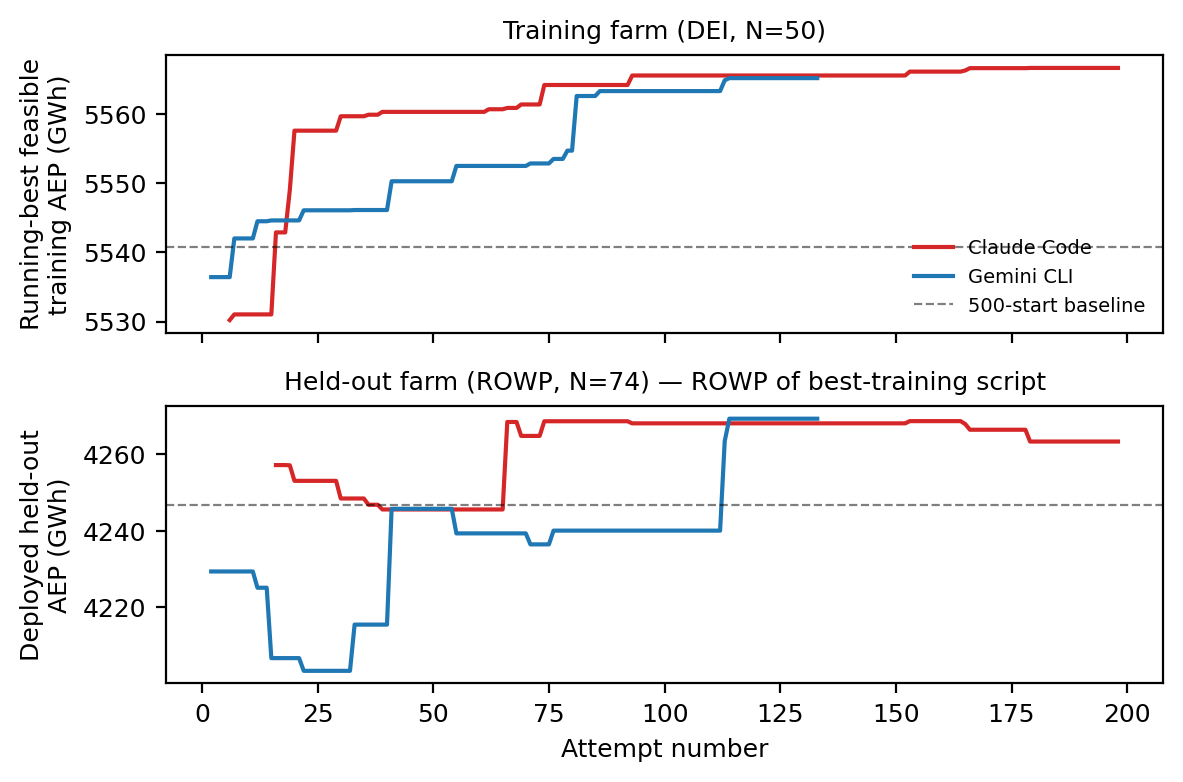
\includegraphics[width=\columnwidth]{figs/fig_short_convergence.png}
\caption{Per-iteration AEP (normalised to final) under Claude
iter\_192, ES-off, K=50 stochastic gradient. Blue: DEI training
($N{=}50$); red: ROWP held-out ($N{=}80$). DEI saturates within
$\sim$1000 iterations; ROWP continues to climb until $\sim$6500
iterations. Vertical line marks the running-max early-stopping
trigger ($\eta_i/\eta_\text{max}\le 0.1$, iter~$\approx$~6440).}
\label{fig:convergence}
\end{figure}

The deployed schedules (\cref{fig:schedules}) use qualitatively
different mechanisms. Claude's \emph{dual Gaussian LR bumps}
temporarily increase the learning rate at $t{=}0.5$ and $t{=}0.75$,
escaping local optima; a coordinated penalty dip at $t{=}0.6$ permits
turbine rearrangement between bumps. Gemini's \emph{8-cycle cosine
restarts} continuously perturb the optimizer with cyclic Adam betas
that reset at each restart, while an aggressive $\alpha$ ramp to
$5{\times}10^6\,\alpha_0$ forces feasibility at convergence. We take ``novel'' to mean: not available as a built-in scheduler in
PyTorch's \texttt{torch.optim.lr\_scheduler} or Optax
(\texttt{optax.schedules}) as of their 2024 releases, and not a
direct instantiation of a named schedule we are aware of in the LR
/ momentum schedule
literature~\cite{loshchilov2017sgdr,smith2017cyclical,smith2019superconvergence,izmailov2018swa,jastrzebski2018factors}.
By that test, neither the dual Gaussian LR bump with coordinated
penalty dip, nor the synchronized cyclic $(\beta_1,\beta_2)$ reset
at cosine-restart boundaries, is available out-of-the-box or
described as a recipe in the cited works. We do not claim
exhaustive novelty; the point is that the agents, given the narrow
interface, compose schedule structures that are not the first thing
a practitioner reaches for.

\begin{figure}[t]
\centering
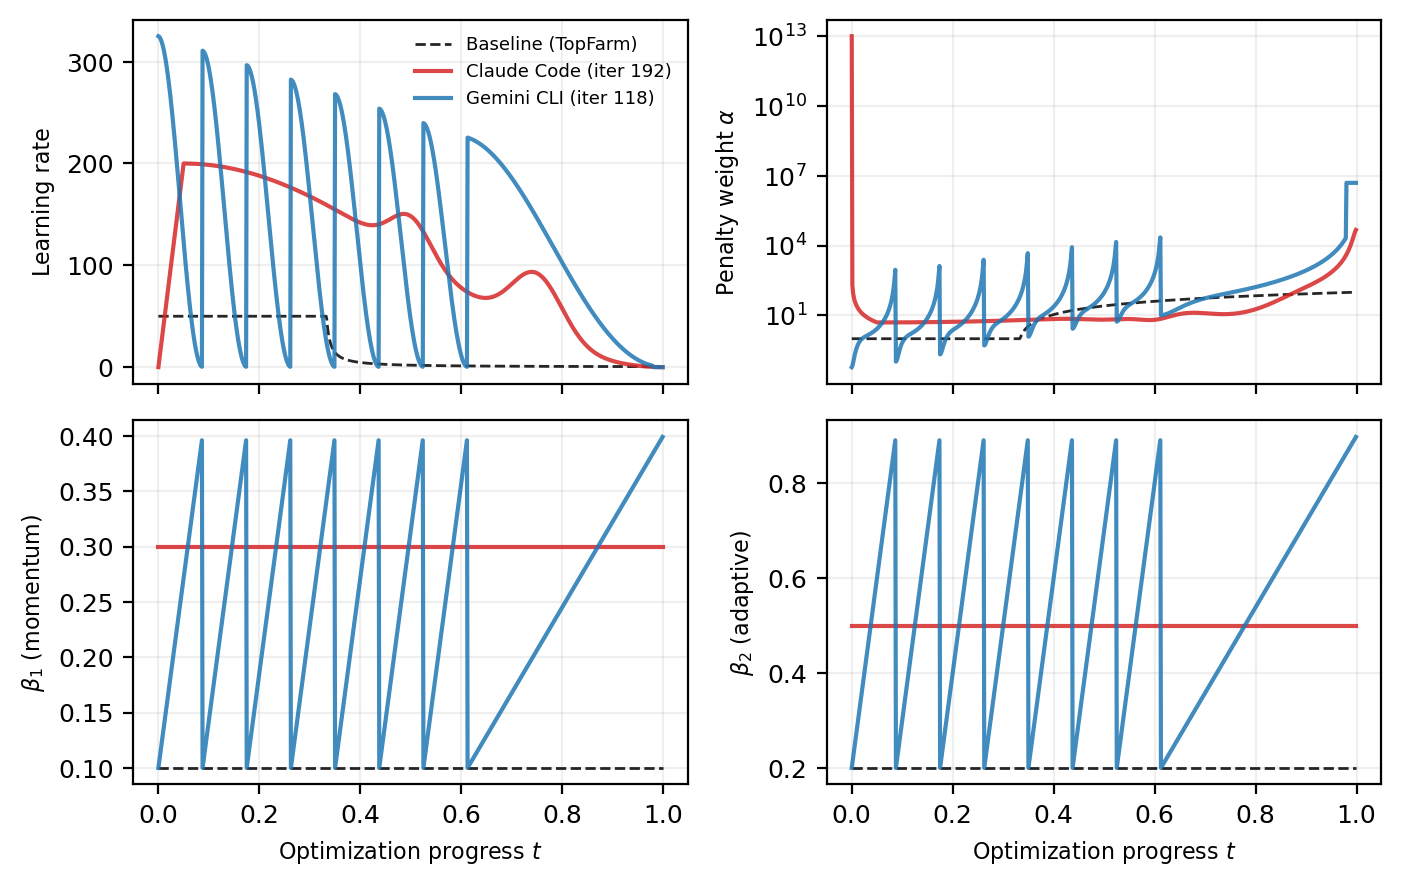
\includegraphics[width=\columnwidth]{figs/fig_short_schedules.png}
\caption{Deployed schedule parameters over optimization progress. The
baseline (dashed) uses monotonic cosine decay with coupled
$\alpha \propto 1/\eta$ and fixed Adam betas. Claude (red) adds dual
Gaussian LR bumps and a penalty dip. Gemini (blue) uses 8-cycle cosine
restarts with cyclic betas and an aggressive terminal penalty ramp.
Note log-scale $\alpha$.}
\label{fig:schedules}
\end{figure}

These schedules generalize across the 64-cell evaluation matrix
(\cref{fig:matrix}): gains increase with packing density ($<1\%$ at
$N{=}30$, up to $0.6\%$ at $N{=}80$) and transfer to the physically
distinct held-out polygon. Schedules discovered at $N{=}50$ (30\,s per
evaluation) generalize to $N{=}200$ (340\,s) without modification,
enabling cheap search and expensive deployment.

\begin{figure*}[t]
\centering
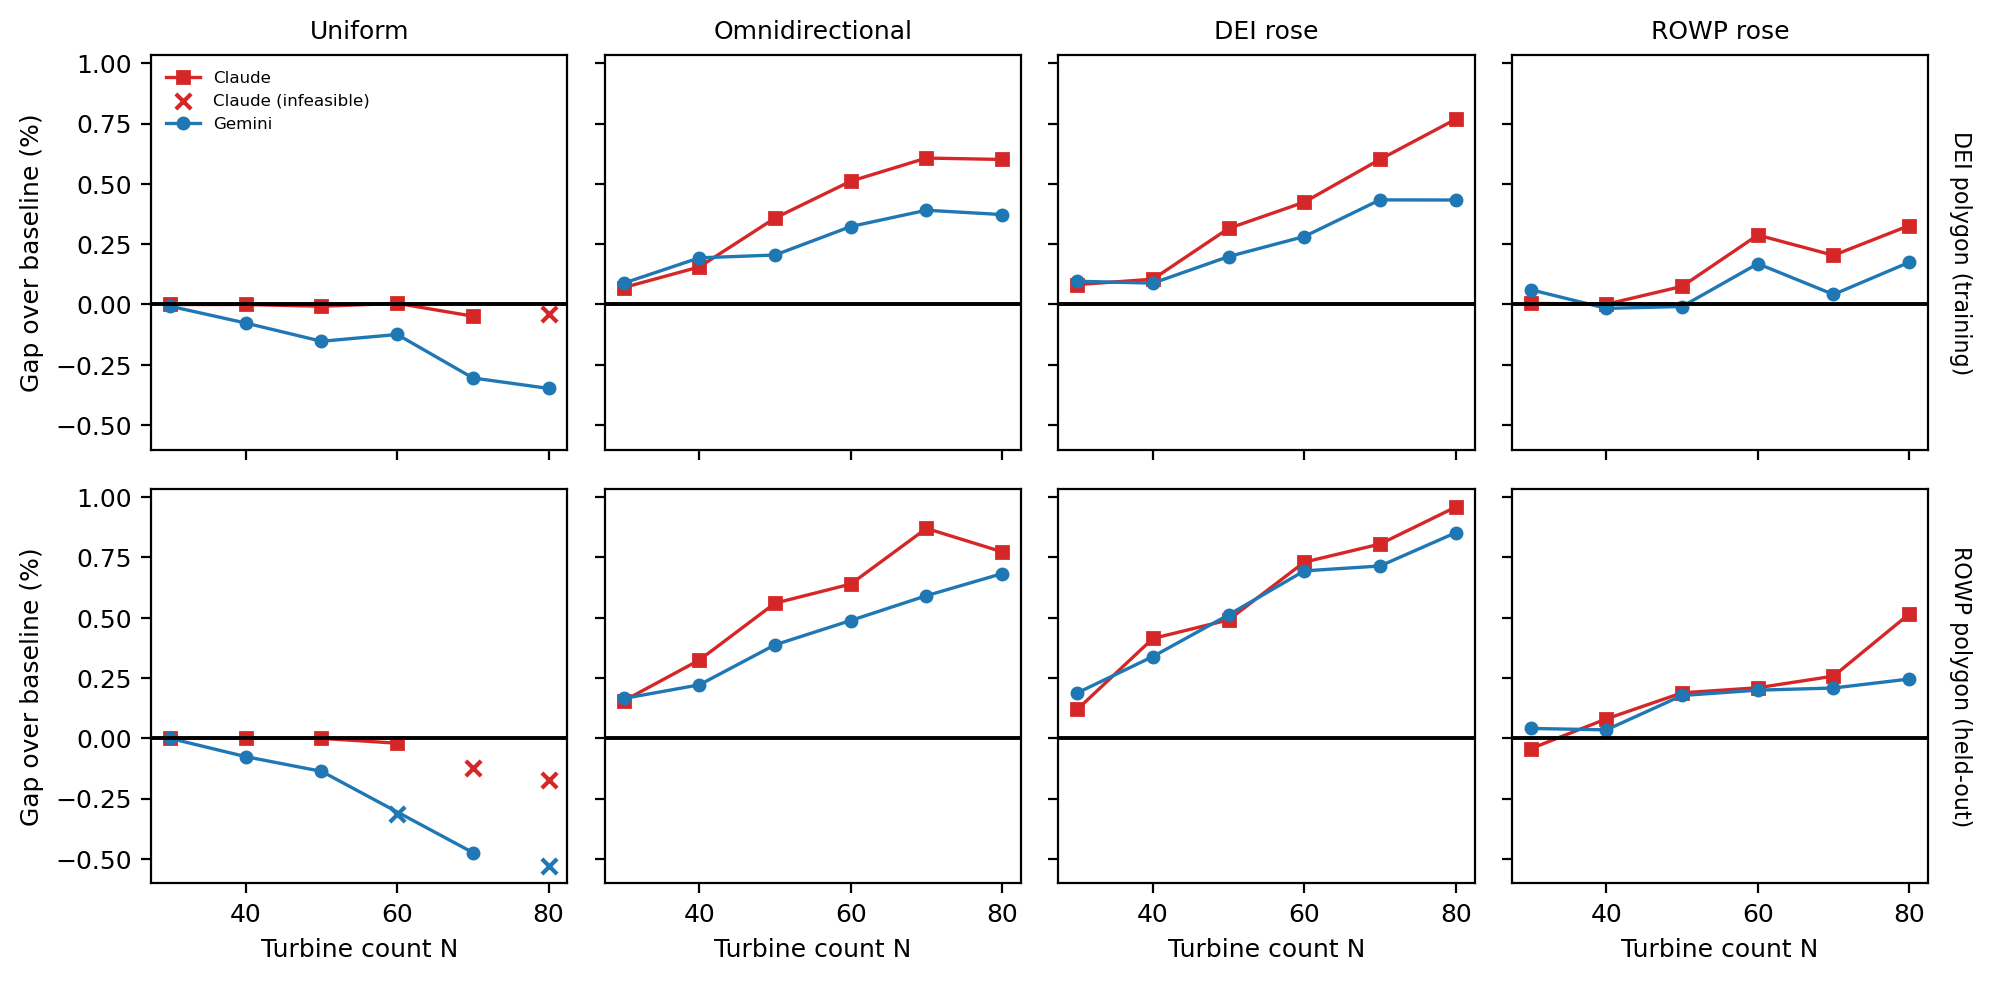
\includegraphics[width=\textwidth]{figs/fig_short_matrix.png}
\caption{Generalization across the evaluation matrix (\% gap over
per-cell 500-start baseline). Top: DEI (training geometry); bottom:
ROWP (held-out). LLM schedules gain most at high $N$. Uniform wind
(column 1) is a failure case: the 1D optimal layout differs
qualitatively from multi-directional cases. A cross ($\times$)
indicates the schedule produced an infeasible layout (violating
boundary or spacing constraints) in that cell; blank cells are
feasible and the color encodes $\Delta$AEP vs.\ baseline.}
\label{fig:matrix}
\end{figure*}

\subsection{Full-Optimizer: Engineering, Not Discovery}

Given the full interface, both agents converge on wrapping
community-standard solvers rather than inventing new algorithms.

Gemini independently rediscovers SLSQP~\cite{kraft1988software}, the
established method in the wind energy community, implementing it with
JAX-computed constraint Jacobians and multi-start hexagonal
initialization. Across five independent seeds with 5-hour budgets,
every Gemini full-optimizer run converges to an SLSQP variant. The
best seed reaches 4272.7\,GWh on the held-out farm, matching the
schedule-only result, but the median (+17.3) and worst (+4.2) are
substantially lower, reflecting high variance in initialization
quality rather than algorithmic innovation.

Claude takes a different path but arrives at a similar outcome. Given
18 scored attempts with evaluation feedback, every script wraps
\texttt{topfarm\_sgd\_solve} with improved initialization strategies:
hexagonal grids aligned to the dominant wind direction, random
perturbations with varying seed, and tuned hyperparameters (higher
learning rates, longer constant-LR phases, stronger penalty weights).
The best wrapper reaches 5559.5\,GWh on training but only 4264.9\,GWh
on the held-out farm, well below the schedule-only result (4271.5).
In a separate run without evaluation feedback, Claude produced 19
scripts that all exceeded the timeout and were never tested during the
5-hour session.

When hot-started from the SLSQP solution, Gemini explores more
creative territory: a JAX-native genetic algorithm with K-means
initialization, surplus-turbine pruning, and Augmented Lagrangian
refinement. This approach reaches 5583.4\,GWh on training (the highest
of any method) and produces feasible held-out layouts, but its best
held-out AEP (4271.9) does not exceed the schedule-only result. The
agent iterates on a given algorithm effectively but does not propose
fundamentally new optimization structures from scratch.

The full-optimizer results (\cref{tab:main}) occasionally match
schedule-only on score but never produce novel optimization
structures. The schedule-only interface forces agents into unfamiliar
territory (the less-explored SGD schedule space) where they discover
novel dynamics. In full-optimizer mode, they retreat to what they
know.

\paragraph{SLSQP does not scale.}
The agents' preference for SLSQP is understandable: it outperforms SGD
at small $N$ (16\,s vs.\ 31\,s at $N{=}50$; \cref{tab:scaling}).
However, SLSQP's per-iteration cost scales poorly with turbine count.
At $N{=}200$, multi-start SLSQP exceeds 1600\,s while the
LLM-discovered schedules finish in approximately 350\,s on the same
hardware (\cref{fig:scaling}). This crossover is consistent with Quick
et al.~\cite{quick2023sgd}, who showed SLSQP's computational cost
exceeds SGD's beyond $N{\approx}225$ while SGD produces 0.3--0.5\%
higher AEP. The schedule-only interface constrains agents to the more
scalable SGD skeleton, forcing discovery of novel schedule structures
rather than reimplementation of SLSQP, which does not scale to the
regime where the discovered schedules are most valuable.

\begin{table}[t]
\caption{Single-seed execution time and total farm AEP (summed over
all $N$ turbines; larger $N$ yields larger totals) by method and farm
size. SLSQP is fastest at small $N$ but exceeds 1600\,s at $N{=}200$;
schedule-only scales predictably.}
\label{tab:scaling}
\vskip 0.1in
\begin{center}
\begin{small}
\begin{sc}
\begin{tabular}{llrrr}
\toprule
& & $N{=}50$ & $N{=}80$ & $N{=}200$ \\
\midrule
\multirow{2}{*}{SLSQP}
& Time (s)  & 16   & 21   & $>$1644 \\
& AEP (GWh) & 5557 & 8836 & ---     \\
\midrule
\multirow{2}{*}{Claude sched.}
& Time (s)  & 31   & 67   & 341   \\
& AEP (GWh) & 5562 & 8827 & 20909 \\
\midrule
\multirow{2}{*}{Gemini sched.}
& Time (s)  & 43   & 83   & 362   \\
& AEP (GWh) & 5553 & 8801 & 20873 \\
\bottomrule
\end{tabular}
\end{sc}
\end{small}
\end{center}
\vskip -0.1in
\end{table}

\begin{figure}[t]
\centering
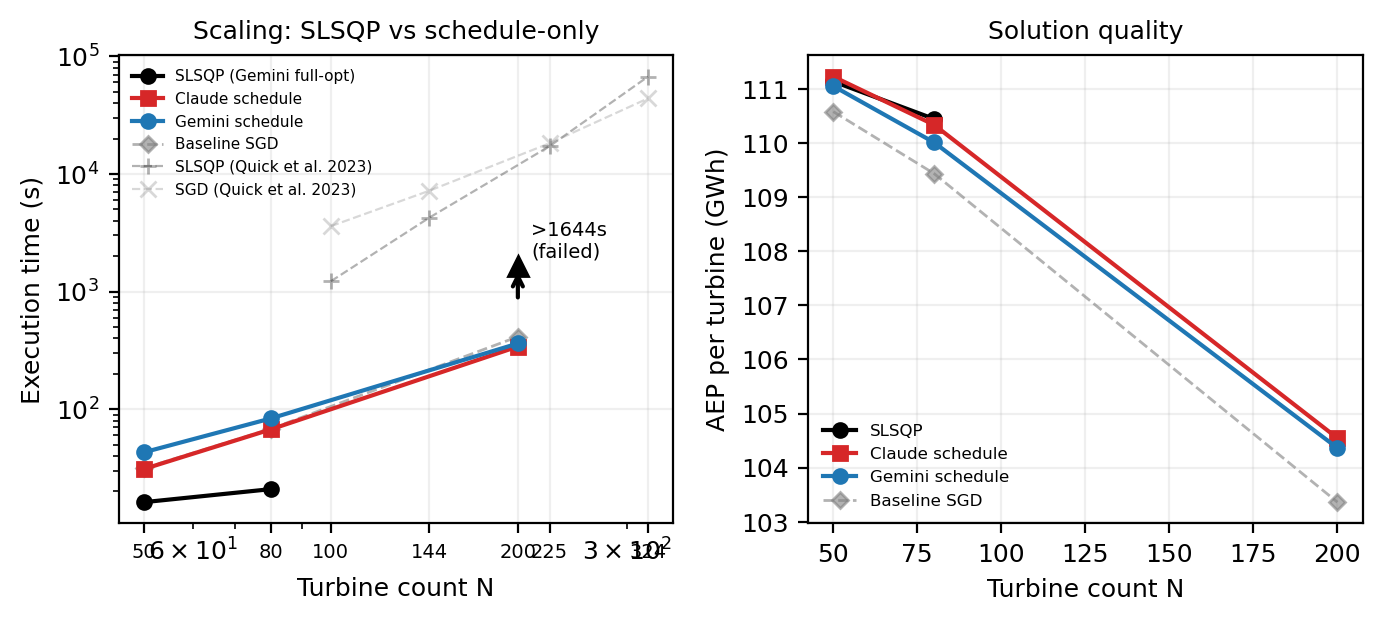
\includegraphics[width=\columnwidth]{figs/fig_short_scaling.png}
\caption{Left: execution time vs.\ turbine count (log-log, same
hardware). SLSQP (black) is fastest at small $N$ but exceeds 1600\,s
at $N{=}200$ ($\blacktriangle$ = lower bound; run did not complete
within 1800\,s). LLM-discovered schedules (red, blue) scale smoothly.
Right: per-turbine AEP; SLSQP has no result at $N{=}200$.}
\label{fig:scaling}
\end{figure}

\subsection{Ablations}

\begin{table*}[t]
\caption{Held-out (ROWP) AEP. Schedule-only rows: mean~$\pm$~std
across 5 initialization seeds, with best/worst seed in brackets;
full-optimizer rows: best/median/worst across 5 agent-run seeds.
$\Delta$ vs.\ 500-start baseline (4246.7\,GWh) using the mean where
available. All schedule-only seeds were 100\% feasible.}
\label{tab:main}
\vskip 0.1in
\begin{center}
\begin{small}
\begin{sc}
\begin{tabular}{lrrr}
\toprule
Method & Train & ROWP & $\Delta$ \\
\midrule
\multicolumn{4}{l}{\emph{Schedule-only (novel structures, 5 init.\ seeds)}} \\
Claude (dual bumps), mean          & 5559.6 & 4266.3 & +19.6 \\
\quad $\pm$std                     & 2.7    & 2.8    &       \\
\quad [best/worst seed]            & [5562.3/5555.4] & [4271.5/4263.5] & \\
Gemini (restarts+squeeze), mean    & 5554.4 & 4262.2 & +15.5 \\
\quad $\pm$std                     & 3.5    & 5.4    &       \\
\quad [best/worst seed]            & [5559.7/5549.6] & [4269.3/4253.9] & \\
\midrule
\multicolumn{4}{l}{\emph{Full-optimizer (known solvers, 5 agent seeds)}} \\
Gemini (SLSQP), best/median/worst  & 5557.1 & 4272.7/4264.0/4250.9 & +26.0/+17.3/+4.2 \\
Claude (SGD wrapper, best/18)      & 5559.5 & 4264.9 & +18.2 \\
\midrule
\multicolumn{4}{l}{\emph{Non-LLM ablation}} \\
Random search (320 samples)        & 5561.8 & 4268.6 & +21.9 \\
\midrule
500-start SGD baseline             & 5540.7 & 4246.7 & ---   \\
\bottomrule
\end{tabular}
\end{sc}
\end{small}
\end{center}
\vskip -0.1in
\end{table*}

Across 5 initialization seeds, both LLM schedules beat the 500-start
baseline on every seed (worst: +16.8\,GWh Claude, +7.2\,GWh Gemini
on ROWP). The schedules the agents selected (based on their single
training evaluation) sit near the \emph{top} of their seed
distributions, indicating mild selection bias: mean performance
(+19.6, +15.5) is 5--7\,GWh below best-seed performance. The ranking
between Claude and Gemini on ROWP is robust across seeds.

Random search inside the LLM-proposed schedule family reaches
4268.6\,GWh ($+21.9$ vs.\ baseline) at matched compute, within
$2$\,GWh of the deployed schedules. The family was designed post-hoc
after inspecting LLM outputs, so this ablation tests whether LLM
structures are findable by random search, not whether random search
would have proposed them.

A controlled ablation varying penalty weight ($0.01\times$ to
$10\times$) while holding LR fixed shows all nine variants produce
feasible held-out layouts under K=50 stochastic gradient (3/3 init
seeds per factor): the LR dynamics drive feasibility. Held-out
AEP is nearly flat across the sweep---feasible-mean spans
4262.9--4267.9\,GWh ($5.0$\,GWh range)---so penalty scale has only
a small effect on quality.

\paragraph{Robust selection across the matrix.}
Selecting the deployed schedule by best training-cell AEP does not
identify the schedule with the best worst-case behavior across the
48 cells of the matrix on which 500-start baselines are computed
(Table~\ref{tab:robust}). All three deployed schedules post
$\Delta\textsc{AEP}\le 0$ or infeasible layouts on three or more
\texttt{*\_roseuniform} cells; selection by worst-cell $\Delta$
would prefer Gemini's restarts-and-squeeze schedule over Claude's
dual-bump schedule, but only because the $N{=}30$ ROWP cells
saturate within $1$\,GWh across all schedules. On every other
non-uniform cell Claude wins. The robust conclusion is that
uniform wind is a \emph{universal} failure mode for SGD-schedule
optimizers under the current FunWake protocol, not that one
discovered schedule is more robust than another. An adversarial
selection rule restricted to non-uniform cells would not change
the deployed-schedule ranking.

\begin{table}[t]
\caption{Worst-cell behavior across the 48-cell matrix subset (single
initialization seed). The worst cell is uniform-wind for all three
deployed schedules. Infeasible cells are excluded from the
worst-cell minimum and reported separately.}
\label{tab:robust}
\vskip 0.1in
\centering
\begin{small}
\begin{sc}
\begin{tabular}{lrrr}
\toprule
Schedule & Train & Worst $\Delta$ & \# infeas \\
\midrule
Claude (iter 179, deploy) & 5560.9 & $-$2.80 & 4 \\
Claude (iter 192, oracle) & 5561.6 & $-$3.80 & 3 \\
Gemini (iter 118)         & 5552.8 & $-$21.84 & 3 \\
\bottomrule
\end{tabular}
\end{sc}
\end{small}
\vskip -0.1in
\end{table}

\paragraph{Adversarial selection in the loop.}
We re-ran the schedule-only loop (codex CLI, \texttt{gpt-5.5},
\texttt{model\_reasoning\_effort=xhigh}) with the deployment
criterion changed to $\min(\text{train\_gap},\
\text{stress\_gap})$, where the stress cell is the dei polygon at
$N{=}50$ with uniform wind --- the documented failure mode in
Table~\ref{tab:robust}. The run terminated at 15 attempts when
the ChatGPT-Codex usage limit was reached. $10/15$ attempts were
feasible on both cells and the in-loop best candidate (iter~014,
tied across iter~008/011/013 at the same \texttt{min\_gap})
reached $\min\_gap=+0.18$\,GWh on the in-loop seed
(Table~\ref{tab:adversarial}). However,
\AdvValSeeds-seed re-evaluation of this candidate shows that the
in-loop positive $\min\_gap$ does \emph{not} survive seed
variation: mean $\min\_gap=\AdvValMinGapMean\pm\AdvValMinGapStd$\,GWh,
matching the \emph{seed-bias} mechanism the original
schedule-only ablations document for Table~\ref{tab:main} but
substantially amplified by the $\min$ rule (the agent can
overfit to lucky seed-induced quirks on either cell).
The result is therefore not a strict improvement over
Table~\ref{tab:main}; it is a Pareto-distinct point: across seeds
the adversarial schedule is feasible on the stress cell
\AdvValBothFeasPct{} of the time
(vs.\ infeasibility or $\Delta\le 0$ for two of the three
schedules in Table~\ref{tab:robust} on \texttt{dei\_n50\_roseuniform}
specifically), and its mean stress-cell $\Delta=\AdvValStressGapMean$\,GWh
sits between Claude iter~192 ($-0.41$) and Gemini iter~118
($-4.78$) on the same cell, while losing roughly $-6$\,GWh on the
training cell. We read this as a methodological finding:
\emph{adversarial selection during agent search requires
multi-seed scoring of every candidate to avoid lucky-seed
artifacts}. With single-seed scoring the agent does find
candidates with a higher rate of stress-cell feasibility than the
original deployments, but the in-loop $\min\_gap$ over-claims;
multi-seed scoring is a clean follow-up that is now compute-bound
rather than codex-bound.

\begin{table}[t]
\caption{Adversarial-selection result. Top: single-seed numbers
from the in-loop deployment (the criterion the agent saw). Bottom:
\AdvValSeeds-seed re-evaluation showing the in-loop $\min\_gap$
does not survive seed variation. All $\Delta$ are vs.\ the
500-start baseline for the corresponding cell
(train $5540.7$\,GWh; stress $5599.79$\,GWh).}
\label{tab:adversarial}
\vskip 0.1in
\centering
\begin{small}
\begin{sc}
\begin{tabular}{lrrr}
\toprule
                                  & Train $\Delta$ & Stress $\Delta$ & min\_gap \\
\midrule
\multicolumn{4}{l}{\emph{In-loop deployment (single seed)}} \\
Codex (iter 014, adv.\ sel.)      & $+$7.37 & $+$0.18 & $+$0.18 \\
\midrule
\multicolumn{4}{l}{\emph{\AdvValSeeds-seed re-evaluation of iter 014}} \\
Mean $\pm$ std                    & \AdvValTrainGapMean$\pm$\AdvValTrainGapStd & \AdvValStressGapMean$\pm$\AdvValStressGapStd & \AdvValMinGapMean$\pm$\AdvValMinGapStd \\
Both-feasible fraction            & \multicolumn{3}{r}{\AdvValBothFeasPct} \\
\bottomrule
\end{tabular}
\end{sc}
\end{small}
\vskip -0.1in
\end{table}

\section{Discussion and Conclusion}

LLM agents discover novel optimizer schedule structures that improve
performance on unseen cases but struggle to design new optimization
algorithms. The schedule-only interface succeeds for two complementary
reasons: it constrains the agent to an unfamiliar search space where
known methods do not apply, and it produces algorithms that scale to
large problem instances where the community-standard SLSQP approach
becomes computationally infeasible.

The interface requires three ingredients: a differentiable physics
simulation, penalty-expressible constraints, and a gradient optimizer.
Topology optimization (SIMP penalty
continuation~\cite{rojas2015continuation}) and trajectory optimization
are immediate candidates for the same benchmark pattern.

\paragraph{Limitations and future work.}
% NOTE (lr0 convention, add if space allows): the skeleton passes a FIXED
% reference learning rate lr0 = 50 m to every schedule on every farm — not
% scaled by rotor diameter or minimum spacing (schedules may reshape it but
% receive no geometry information). Relative to geometry: ~0.21 D on DEI,
% 0.25 D on ROWP, 0.63 D on ParqueFicticio — the Parque transfer test is
% therefore also a step-size out-of-distribution test, likely contributing
% to the degraded transfer there (TopFarm convention scales lr with D).
% Frozen: discovery runs consumed this exact skeleton; changing it means
% re-running the search. Evidence: playground/skeleton.py:102 (lr0=50.0),
% parqo/skeleton_multizone.py:96 (same), run_with_schedule has no lr0 arg.
\emph{Agent-run asymmetry.} Of the four (agent $\times$ interface)
cells in the study, only Gemini $\times$ full-optimizer has
$n{=}5$ agent-run seeds; Claude $\times$ full-optimizer, Claude
$\times$ schedule-only, and Gemini $\times$ schedule-only are
$n{=}1$ each. Our 5-seed evaluation of the best Claude and Gemini
schedules measures initialization variance only. Re-running the
5-hour agent loop with different RNG seeds (budget
$\approx$20~GPU-hrs per cell) is left to follow-up work.
\emph{Scaffold confound.} The narrow-interface agents and the
broad-interface agents used different scaffolds (structured-output
harness vs.\ full CLI). The experiment that would cleanly isolate
interface from scaffold is: run each agent under each scaffold on
each interface. We view this as the most important follow-up before
the narrow-vs-broad causal claim can be promoted from suggestive to
conclusive. Other open items: single training farm ($N{=}1$
held-out polygon); post-hoc random-search family design; per-seed
uniform-wind behavior not resolved.

\paragraph{Reproducibility.}
Claude Code CLI v1.x and Gemini CLI with \texttt{gemini-2.5-flash}
(snapshot retrieved March--April 2026) were used; exact versions,
prompts, and generated scripts are released with the code.

\section*{Impact Statement}

This paper presents work whose goal is to advance the field of Machine
Learning. There are many potential societal consequences of our work,
none which we feel must be specifically highlighted here.

\bibliographystyle{icml2026}
\bibliography{references}

\end{document}
